\documentclass[aspectratio=169, 11pt]{beamer}

% --- Packages & Setup ---
\usepackage[utf8]{inputenc}
\usepackage[T1]{fontenc}
\usepackage{xcolor}
\usepackage{booktabs}
\usepackage{array}
\usepackage{graphicx}
\usepackage{tikz}
\usepackage{pgfplots}
\pgfplotsset{compat=1.17}
\usetikzlibrary{calc,arrows.meta,positioning,shapes.geometric}

\graphicspath{{../}{./}}

% Try loading Open Sans; fallback if missing
\IfFileExists{opensans.sty}{\usepackage[default,scale=0.95]{opensans}}{}

% --- Branding Colors ---
\definecolor{amritaMaroon}{HTML}{A4123F}
\definecolor{maroonSoft}{HTML}{F6E3E9}
\definecolor{inkGray}{HTML}{3A3A3A}
\definecolor{goldAccent}{HTML}{C79A3A}

% --- Theme Setup ---
\usetheme{Madrid}
\usecolortheme[named=amritaMaroon]{structure}
\setbeamertemplate{navigation symbols}{}
\setbeamertemplate{footline}[frame number]
\setbeamertemplate{bibliography item}[text]

% node styles reused across diagrams
\tikzset{
  lbl/.style={circle, draw=amritaMaroon, thick, fill=maroonSoft, minimum size=1.05cm, font=\scriptsize, align=center},
  lblcenter/.style={circle, draw=amritaMaroon, very thick, fill=amritaMaroon, text=white, minimum size=1.15cm, font=\bfseries\scriptsize, align=center},
  edg/.style={-, thick, draw=inkGray},
  edgfaint/.style={-, draw=inkGray!35},
  edghi/.style={-, ultra thick, draw=amritaMaroon},
  stepbox/.style={rectangle, draw=amritaMaroon, thick, fill=maroonSoft, rounded corners=2pt, minimum width=3.4cm, minimum height=0.75cm, font=\footnotesize, align=center},
  notebox/.style={rectangle, draw=amritaMaroon, very thick, fill=maroonSoft, rounded corners=3pt, inner sep=8pt, align=left},
  checkitem/.style={rectangle, draw=amritaMaroon, thick, fill=maroonSoft, rounded corners=2pt, minimum width=4.6cm, minimum height=0.9cm, font=\footnotesize, align=center}
}

% small icon-in-circle helpers for the Applications slide
\newcommand{\iconGraph}{%

\begin{tikzpicture}
\node[circle, fill=amritaMaroon, minimum size=0.9cm] (bg) {};
\node[circle, fill=white, minimum size=0.11cm, inner sep=0pt] (a) at ($(bg.center)+(-0.18,0.15)$) {};
\node[circle, fill=white, minimum size=0.11cm, inner sep=0pt] (b) at ($(bg.center)+(0.18,0.15)$) {};
\node[circle, fill=white, minimum size=0.11cm, inner sep=0pt] (c) at ($(bg.center)+(0,-0.2)$) {};
\draw[white, thin] (a) -- (b) -- (c) -- (a);
\end{tikzpicture}}

\newcommand{\iconMagnify}{%

\begin{tikzpicture}
\node[circle, fill=amritaMaroon, minimum size=0.9cm] (bg) {};
\draw[white, thick] ($(bg.center)+(-0.05,0.1)$) circle (0.17cm);
\draw[white, thick, line cap=round] ($(bg.center)+(0.07,-0.02)$) -- ($(bg.center)+(0.27,-0.24)$);
\end{tikzpicture}}

\newcommand{\iconDNA}{%

\begin{tikzpicture}
\node[circle, fill=amritaMaroon, minimum size=0.9cm] (bg) {};
\draw[white, thick] ($(bg.center)+(-0.2,0.28)$) .. controls ($(bg.center)+(0.2,0.12)$) and ($(bg.center)+(-0.2,-0.12)$) .. ($(bg.center)+(0.2,-0.28)$);
\draw[white, thick] ($(bg.center)+(0.2,0.28)$) .. controls ($(bg.center)+(-0.2,0.12)$) and ($(bg.center)+(0.2,-0.12)$) .. ($(bg.center)+(-0.2,-0.28)$);
\end{tikzpicture}}

\newcommand{\iconLeaf}{%

\begin{tikzpicture}
\node[circle, fill=amritaMaroon, minimum size=0.9cm] (bg) {};
\draw[white, thick] ($(bg.center)+(0,-0.3)$) -- ($(bg.center)+(0,0.05)$);
\filldraw[white] ($(bg.center)+(0.02,0.2)$) ellipse[x radius=0.22cm, y radius=0.13cm, rotate=40];
\draw[amritaMaroon, thin] ($(bg.center)+(-0.13,0.11)$) -- ($(bg.center)+(0.17,0.29)$);
\end{tikzpicture}}

\newcommand{\iconCheck}{%

\begin{tikzpicture}
\node[circle, fill=amritaMaroon, minimum size=0.6cm] (bg) {};
\draw[white, very thick, line cap=round, line join=round]
  ($(bg.center)+(-0.14,0)$) -- ($(bg.center)+(-0.03,-0.13)$) -- ($(bg.center)+(0.17,0.15)$);
\end{tikzpicture}}

\begin{document}

% ============================================================
% FRAME: What is the WL Graph Kernel?
% ============================================================
\begin{frame}{What is the WL Graph Kernel?}
    % \framesubtitle{Weisfeiler--Lehman (WL) Graph Kernel}
    \begin{columns}[c]
        \column{0.52\textwidth}
        \textbf{Main idea}
        \vspace{0.15cm}

        The Weisfeiler--Lehman (WL) graph kernel \cite{shervashidze2011weisfeiler} compares graphs by \textbf{iteratively capturing the
        labels of each node and its neighborhood} (rooted in the 1-WL isomorphism test \cite{weisfeiler1968reduction}).

        \vspace{0.3cm}
        \begin{itemize}
            \item Every node starts with a simple label.
            \item Labels are repeatedly updated using neighboring labels.
            \item The resulting label patterns are turned into a
            feature vector used to measure \textbf{similarity between graphs}.
        \end{itemize}

        \column{0.44\textwidth}
        \centering
        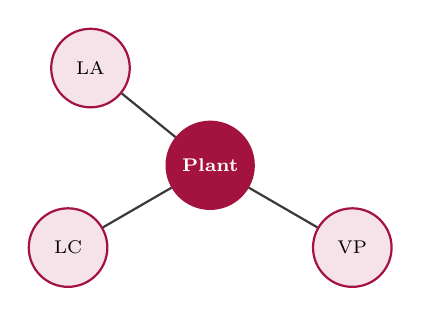
\begin{tikzpicture}[scale=0.95, every node/.style={transform shape}]
            \node[lblcenter] (p) at (0,0) {Plant};
            \node[lbl] (la) at (-1.6,1.3) {LA};
            \node[lbl] (lc) at (-1.9,-1.1) {LC};
            \node[lbl] (vp) at (1.9,-1.1) {VP};
            \draw[edg] (p) -- (la);
            \draw[edg] (p) -- (lc);
            \draw[edg] (p) -- (vp);
        \end{tikzpicture}

        \vspace{0.1cm}
        {\scriptsize\itshape A node's label evolves by absorbing
        information from its neighbors.}
    \end{columns}
\end{frame}

% ============================================================
% FRAME: How Does WL Work? -- Visual Demonstration
% ============================================================
\begin{frame}{How Does WL Work?}

    \begin{center}
        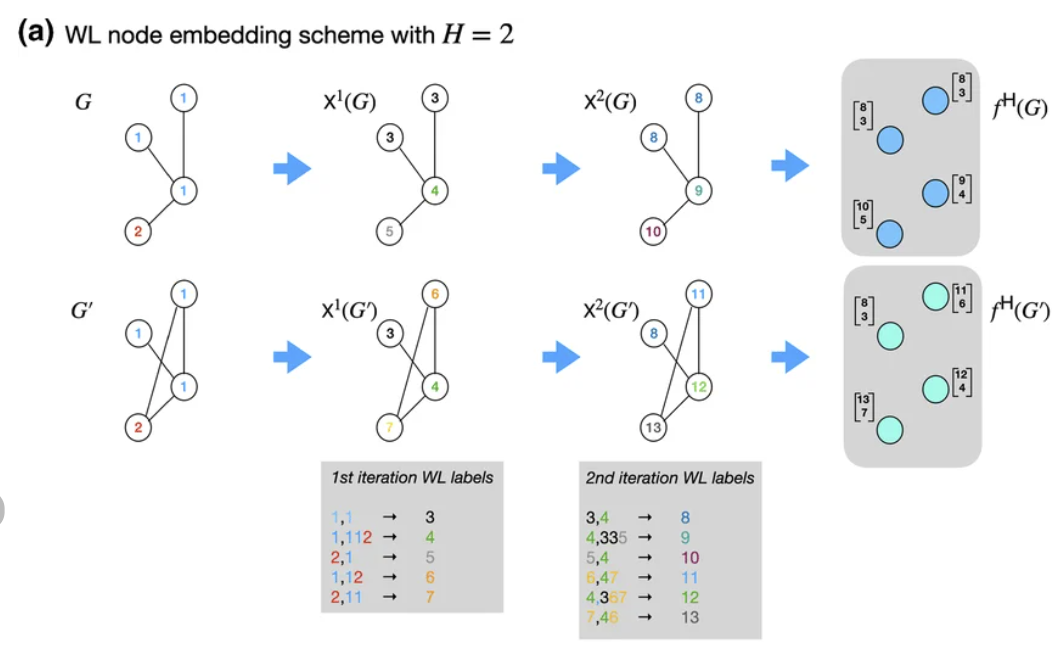
\includegraphics[width=0.85\textwidth, height=0.75\textheight, keepaspectratio]{wl_demo.png}
    \end{center}

    \vspace{-0.15cm}
    \begin{center}
        {\scriptsize\itshape Subtree neighborhood aggregation in the Weisfeiler--Lehman framework \cite{shervashidze2011weisfeiler}.}
    \end{center}

    \note{The main technique used in this research is the Weisfeiler--Lehman graph
    kernel \cite{shervashidze2011weisfeiler}. WL starts with the labels of the nodes and iteratively updates each
    node's label based on its own label and the labels of its neighbors.}
\end{frame}


% ============================================================
% FRAME: WL Algorithm -- Mathematical Formulation
% ============================================================
\begin{frame}{WL Algorithm: Mathematical Formulation}
    \framesubtitle{The formal update rule behind the visual picture \cite{weisfeiler1968reduction, shervashidze2011weisfeiler}}

    \begin{center}
        \Large
        $$ l_i(v) = f\left(l_{i-1}(v),\ \{\!\{\, l_{i-1}(u) : u \in N(v) \,\}\!\}\right) $$
    \end{center}

    \vspace{0.2cm}
    \begin{itemize}
        \item $l_i(v)$ -- the label of node $v$ after iteration $i$.
        \item $l_{i-1}(v)$ -- the node's own label from the previous iteration.
        \item $N(v)$ -- the set of neighbors of $v$.
        \item $\{\!\{\, l_{i-1}(u) : u \in N(v) \,\}\!\}$ -- the \textbf{multiset}
        of neighbor labels (order doesn't matter, repeats are kept).
        \item $f$ -- a hashing/compression function that combines a node's own
        label with its neighbors' labels into a new, compact label \cite{shervashidze2011weisfeiler}.
    \end{itemize}

    \vspace{0.15cm}

\end{frame}



% ============================================================
% FRAME: Applications in the Literature (evidence slide)
% ============================================================
\begin{frame}{Applications in the Literature}
    \framesubtitle{WL graph kernels power real detection and comparison systems}

    \begin{center}
    \begin{tikzpicture}[every node/.style={transform shape}]
        \node[anchor=north west, inner sep=0] (img1) at (0,0)
            {\includegraphics[width=3.5cm]{img1_malware.png}};
        \node[anchor=north west, text width=7.7cm, align=left] (txt1) at (4.0,0.05) {
            \footnotesize\textbf{Malware Detection}\\[2pt]
            \scriptsize A \emph{contextual} WL graph kernel over program
            behavior graphs distinguishes malware from benign software
            \cite{narayanan2016contextual}.
        };

        \node[anchor=north west, inner sep=0] (img2) at (0,-2.0)
            {\includegraphics[width=3.5cm]{img2_program.png}};
        \node[anchor=north west, text width=7.7cm, align=left] (txt2) at (4.0,-1.95) {
            \footnotesize\textbf{Program Similarity Detection}\\[2pt]
            \scriptsize The WL kernel compares program graphs directly to
            detect similar or cloned code, without hand-crafted features
            \cite{li2016detecting}.
        };

        \node[anchor=north west, inner sep=0] (img3) at (0,-4.0)
            {\includegraphics[width=3.5cm]{img3_bioinfo.png}};
        \node[anchor=north west, text width=7.7cm, align=left] (txt3) at (4.0,-3.95) {
            \footnotesize\textbf{Bioinformatics -- Protein Function}\\[2pt]
            \scriptsize Amino-acid-level protein graphs, scored with WL
            kernels, support \textbf{protein function} and phenotype
            prediction \cite{borgwardt2005protein, shervashidze2011weisfeiler} -- the same principle used here for plant traits.
        };
    \end{tikzpicture}
    \end{center}

    \vspace{0.05cm}
    {\scriptsize\itshape Across security, software engineering, and biology,
    the same idea recurs: represent structure as a graph, let WL capture
    its neighborhoods, and compare.}
\end{frame}

% ============================================================
% FRAME: How Does the WL Graph Kernel Perform Classification?
% ============================================================
\begin{frame}{How Does the WL Graph Kernel Perform Classification?}
    \begin{center}
    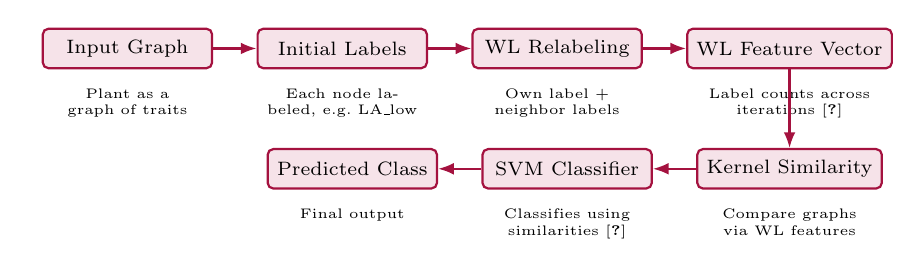
\begin{tikzpicture}[every node/.style={transform shape}]
        \tikzset{
            wlbox/.style={rectangle, draw=amritaMaroon, thick, fill=maroonSoft,
                rounded corners=2pt, minimum width=2.15cm, minimum height=0.5cm,
                font=\scriptsize, align=center},
            wlcap/.style={font=\tiny, align=center, text width=2.3cm}
        }
        % Row 1: left to right
        \node[wlbox] (b1) at (0,0) {Input Graph};
        \node[wlbox, right=0.55cm of b1] (b2) {Initial Labels};
        \node[wlbox, right=0.55cm of b2] (b3) {WL Relabeling};
        \node[wlbox, right=0.55cm of b3] (b4) {WL Feature Vector};

        \node[wlcap, below=0.12cm of b1] (c1) {Plant as a graph of traits};
        \node[wlcap, below=0.12cm of b2] (c2) {Each node labeled, e.g.\ LA\_low};
        \node[wlcap, below=0.12cm of b3] (c3) {Own label + neighbor labels};
        \node[wlcap, below=0.12cm of b4] (c4) {Label counts across iterations \cite{shervashidze2011weisfeiler}};

        % Row 2: right to left, continuing the flow
        \node[wlbox, below=1.0cm of b4] (b5) {Kernel Similarity};
        \node[wlbox, left=0.55cm of b5] (b6) {SVM Classifier};
        \node[wlbox, left=0.55cm of b6] (b7) {Predicted Class};

        \node[wlcap, below=0.12cm of b5] (c5) {Compare graphs via WL features};
        \node[wlcap, below=0.12cm of b6] (c6) {Classifies using similarities \cite{cortes1995support}};
        \node[wlcap, below=0.12cm of b7] (c7) {Final output};

        \draw[-{Latex[length=2mm]}, thick, draw=amritaMaroon] (b1) -- (b2);
        \draw[-{Latex[length=2mm]}, thick, draw=amritaMaroon] (b2) -- (b3);
        \draw[-{Latex[length=2mm]}, thick, draw=amritaMaroon] (b3) -- (b4);
        \draw[-{Latex[length=2mm]}, thick, draw=amritaMaroon] (b4) -- (b5);
        \draw[-{Latex[length=2mm]}, thick, draw=amritaMaroon] (b5) -- (b6);
        \draw[-{Latex[length=2mm]}, thick, draw=amritaMaroon] (b6) -- (b7);
    \end{tikzpicture}
    \end{center}

  
\end{frame}


% ============================================================
% FRAME: Dataset -- OLID Leaf Image Dataset
% ============================================================
\begin{frame}{Dataset: OLID Leaf Image Dataset}


    \begin{columns}[c]
        \column{0.5\textwidth}
        \textbf{Source}
        \begin{itemize}
            \item \textbf{OLID} -- Open Leaf Image Dataset \cite{orka2023olid}
            \item \textbf{21\,GB} of raw images
            \item Approximately \textbf{4{,}749 images} across multiple crops
        \end{itemize}

        \vspace{0.2cm}


        \column{0.46\textwidth}
        \centering
        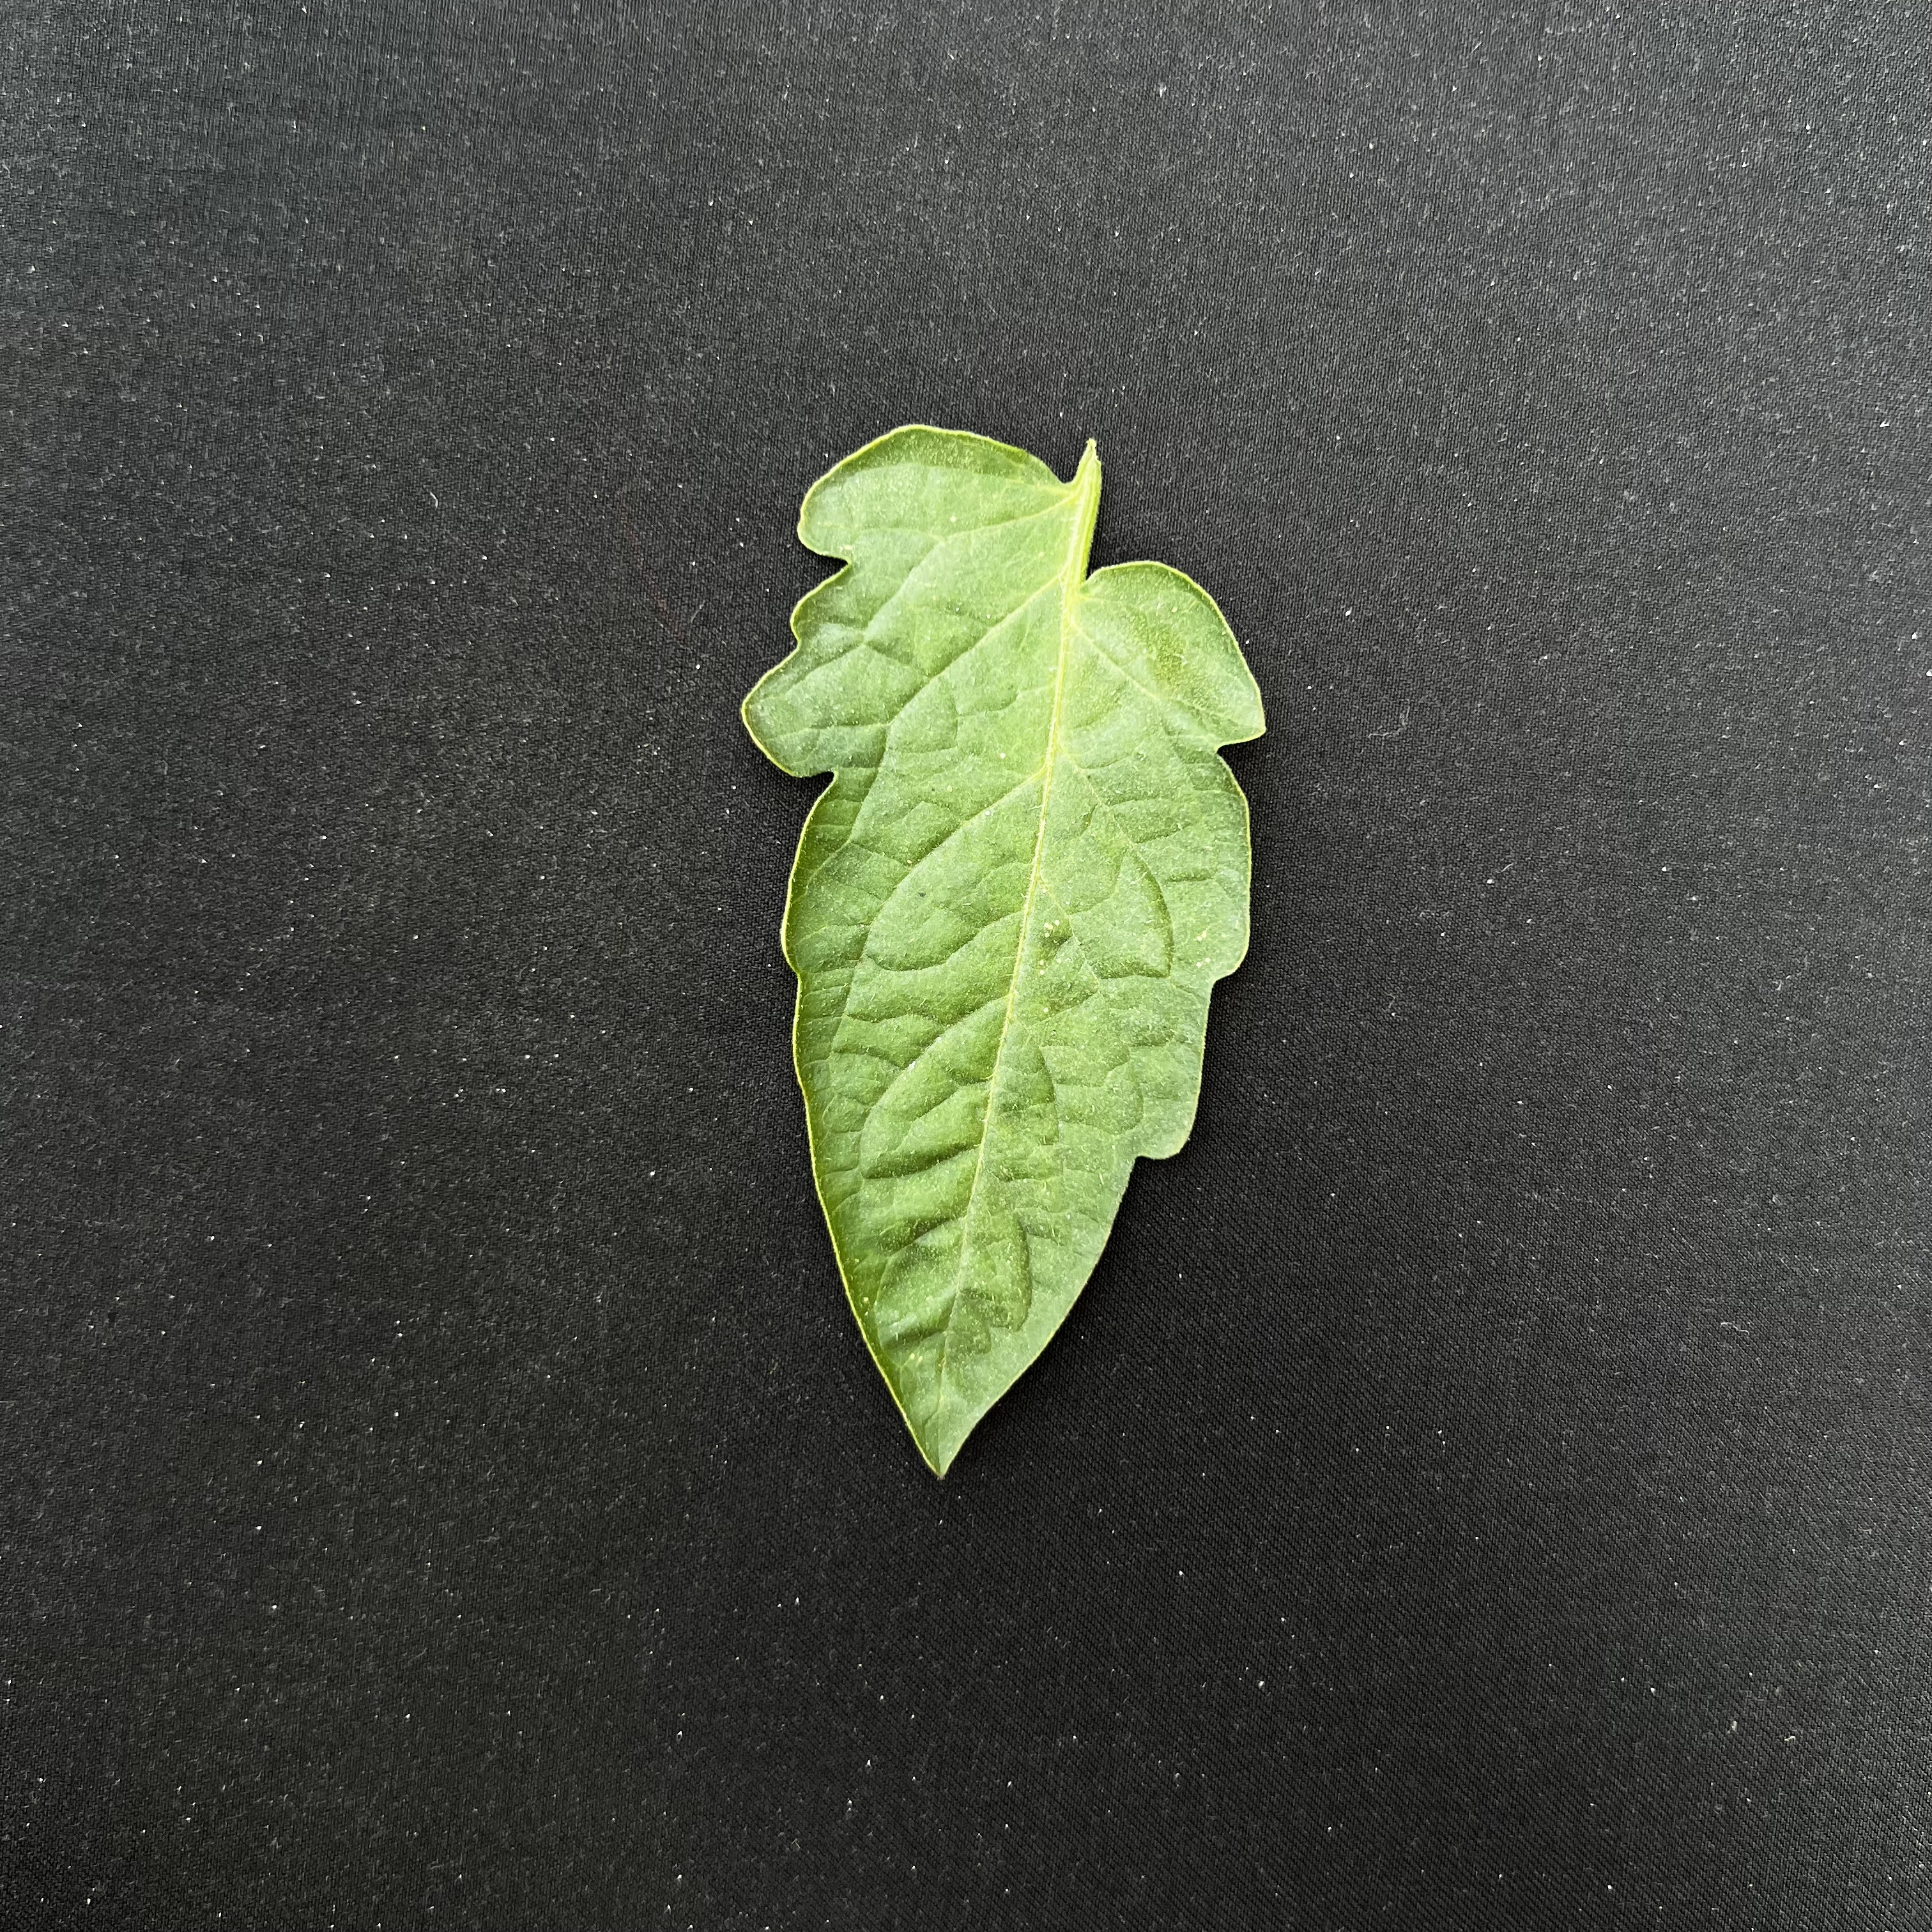
\includegraphics[width=0.85\textwidth]{leaf_sample.JPG}\\
        {\scriptsize\itshape Sample raw leaf image}
    \end{columns}
\end{frame}

% ============================================================
% FRAME: Preprocessing -- Segmentation
% ============================================================
\begin{frame}{Preprocessing: Leaf Segmentation}
    \framesubtitle{Separating the leaf from the background}

    \begin{columns}[c]
        \column{0.48\textwidth}
        \textbf{ExG (Excess Green) segmentation \cite{woebbecke1995color}}
        \begin{itemize}
            \item Computes an Excess Green index ($2G - R - B$) over the RGB image to
            highlight vegetation \cite{woebbecke1995color}.
            \item The mask isolates the leaf pixels from the background,
            independent of lighting or backdrop color.
        \end{itemize}

        \column{0.5\textwidth}
        \centering
        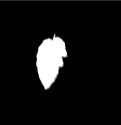
\includegraphics[width=\textwidth]{segmentation_example.png}\\[0.15cm]
        {\scriptsize\itshape Raw leaf image $\rightarrow$ Segmentation
        $\rightarrow$ binary leaf mask}
    \end{columns}
\end{frame}

% ============================================================
% FRAME: Feature Extraction -- 38 Extracted Features
% ============================================================
\begin{frame}{Feature Extraction: 38 Features}
    \framesubtitle{Every leaf is described by a 38-dimensional feature set}

    \tiny
    \renewcommand{\arraystretch}{1.15}
    \begin{center}
    \begin{tabular}{@{}p{2.7cm}p{2.6cm}p{2.4cm}p{2.4cm}@{}}
        \toprule
        \textbf{Shape \& Geometry (10)} & \textbf{RGB (6)} & \textbf{HSV (6)} & \textbf{Lab (6)} \\
        \midrule
        Area & Mean R & Mean H & Mean L \\
        Perimeter & Std R & Std H & Std L \\
        Aspect Ratio & Mean G & Mean S & Mean a \\
        Circularity & Std G & Std S & Std a \\
        Extent & Mean B & Mean V & Mean b \\
        Solidity & Std B & Std V & Std b \\
        Convex Area & & & \\
        Major Axis Length & & & \\
        Minor Axis Length & & & \\
        Eccentricity & & & \\
        \bottomrule
    \end{tabular}

    \vspace{0.15cm}
    \begin{tabular}{@{}p{2.9cm}p{3.4cm}p{3.4cm}@{}}
        \toprule
        \textbf{Derived Color (2)} & \textbf{Texture -- GLCM \cite{haralick1973textural} (4)} & \textbf{Spatial / Regional (4)} \\
        \midrule
        Green Ratio & Contrast & Core Mean H \\
        Yellow Ratio & Homogeneity & Core Yellow Ratio \\
        & Energy & Edge Mean H \\
        & Correlation & Edge Yellow Ratio \\
        \bottomrule
    \end{tabular}
    \end{center}

    \vspace{0.15cm}
    \normalsize
    \begin{center}
    {\footnotesize\bfseries Each of these 38 features is represented as a
    node in our graph.}
    \end{center}
\end{frame}


% ============================================================
% FRAME: Feature Validation -- Acceptance Rule
% ============================================================
% ============================================================
% FRAME: Feature Validation -- Acceptance Rule
% ============================================================
\begin{frame}{Feature Validation: Basis for Acceptance}


    \textbf{Otsu-based Exclusion Mechanism \cite{otsu1979threshold}}
    \vspace{0.15cm}

    {\footnotesize Discards distorted segmentations by checking the extracted binary mask against physical bounds:}

    \vspace{0.2cm}
    \begin{center}
    \begin{tikzpicture}
        \node[stepbox, minimum width=8cm, minimum height=1cm, font=\normalsize] {
            $\text{Mask Area Ratio} = \dfrac{\text{Leaf mask area}}{\text{Total image area}}$
        };
    \end{tikzpicture}
    \end{center}

    \vspace{0.2cm}
    {\footnotesize Acceptance rules applied per leaf instance:}

    \vspace{0.1cm}
    \small
    \begin{center}
    \begin{tabular}{@{}lll@{}}
        \toprule
        \textbf{Condition} & \textbf{Status} & \textbf{Meaning} \\
        \midrule
        $\text{ratio} < 0.01 \text{ or } \text{ratio} = 0$ & \textcolor{amritaMaroon}{\bfseries FAILED} & Almost no leaf detected \\
        $\text{ratio} > 0.98$ & \textcolor{goldAccent}{\bfseries SUSPICIOUS} & Almost the entire image detected as leaf \\
        $0.01 \le \text{ratio} \le 0.98$ & \textbf{ACCEPT} & Segmentation is considered reasonable \\
        \bottomrule
    \end{tabular}
    \end{center}
\end{frame}

% ============================================================
% FRAME: Segmentation Validation Examples
% ============================================================
\begin{frame}{Segmentation Validation Examples}
    \framesubtitle{Visualizing acceptance and rejection criteria via Otsu-based masking \cite{otsu1979threshold}}

    \begin{columns}[T]
        % --- ACCEPTED COLUMN ---
        \column{0.48\textwidth}
        \centering
        \textbf{\textcolor{green!60!black}{Accepted Samples} ($0.01 \leq \text{Ratio} \leq 0.98$)}
        \vspace{0.25cm}

        \begin{tikzpicture}
            % Sample 1: Accepted
            \node[inner sep=0, draw=green!60!black, very thick] (imgA1) at (0, 0)
                {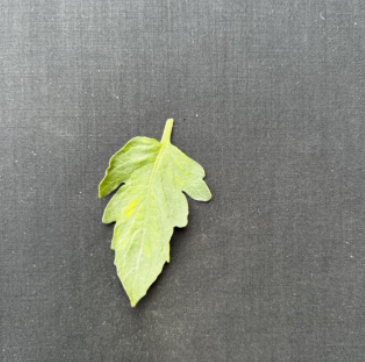
\includegraphics[width=2.5cm, height=1.7cm]{accepted_leaf1.png}};
            \node[below=0.08cm of imgA1, font=\tiny, align=center] {
                \textbf{Sample 1:} Ratio $\approx 0.0759$ \\
                % Clean boundary \& distinct leaf
            };

            % Sample 2: Accepted
            \node[inner sep=0, draw=green!60!black, very thick] (imgA2) at (0, -2.55)
                {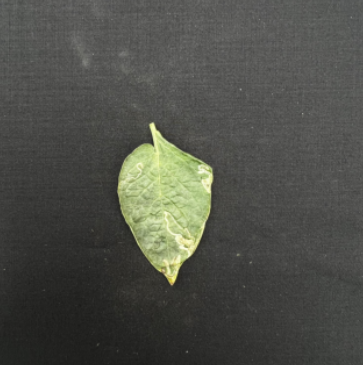
\includegraphics[width=2.5cm, height=1.7cm]{accepted_leaf2.png}};
            \node[below=0.08cm of imgA2, font=\tiny, align=center] {
                \textbf{Sample 2:} Ratio $\approx 0.1542$ \\
                % Valid morphology, robust foreground
            };
        \end{tikzpicture}

        % --- DECLINED COLUMN ---
        \column{0.48\textwidth}
        \centering
        \textbf{\textcolor{red}{Declined Samples} ($\text{Ratio} < 0.01$ or $> 0.98$)}
        \vspace{0.25cm}

        \begin{tikzpicture}
            % Sample 1: Under-segmentation / Empty
            \node[inner sep=0, draw=red, very thick] (imgD1) at (0, 0)
                {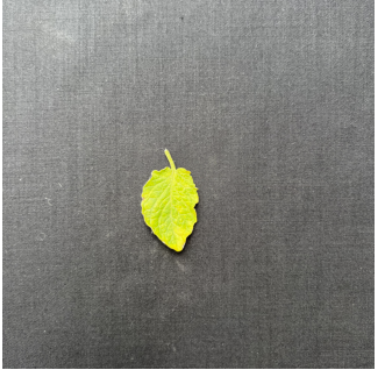
\includegraphics[width=2.5cm, height=1.7cm]{declined_empty.png}};
            \node[below=0.08cm of imgD1, font=\tiny, align=center] {
                \textbf{Over-segmented:} Ratio $= 0.99$ \\
                
            };

            % Sample 2: Over-segmentation / Artifact
            \node[inner sep=0, draw=red, very thick] (imgD2) at (0, -2.55)
                {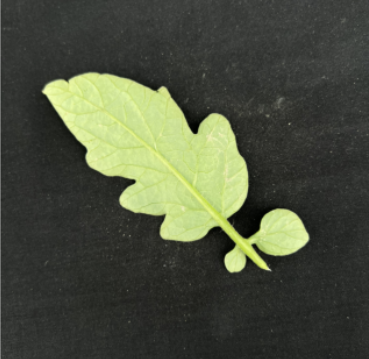
\includegraphics[width=2.5cm, height=1.7cm]{declined_flooded.png}};
            \node[below=0.08cm of imgD2, font=\tiny, align=center] {
                \textbf{Under-segmented:} Ratio $= 0.0002$ \\
                Tiny Mask
            };
        \end{tikzpicture}
    \end{columns}

    \vspace{0.15cm}
    \begin{center}
        {\tiny\itshape Replace \texttt{accepted\_leaf1.png}, \texttt{accepted\_leaf2.png}, \texttt{declined\_empty.png}, and \texttt{declined\_flooded.png} with your actual image paths.}
    \end{center}
\end{frame}


% ============================================================
% FRAME: Segmentation & Feature Sanity Checks
% ============================================================
\begin{frame}{Segmentation & Feature Sanity Checks}
    \framesubtitle{Validating the dataset before graph construction}

    \begin{columns}[c]
        
        % Left: Acceptance
        \column{0.50\textwidth}
        \centering
        \textbf{Segmentation Acceptance by Crop}\\[6pt]
        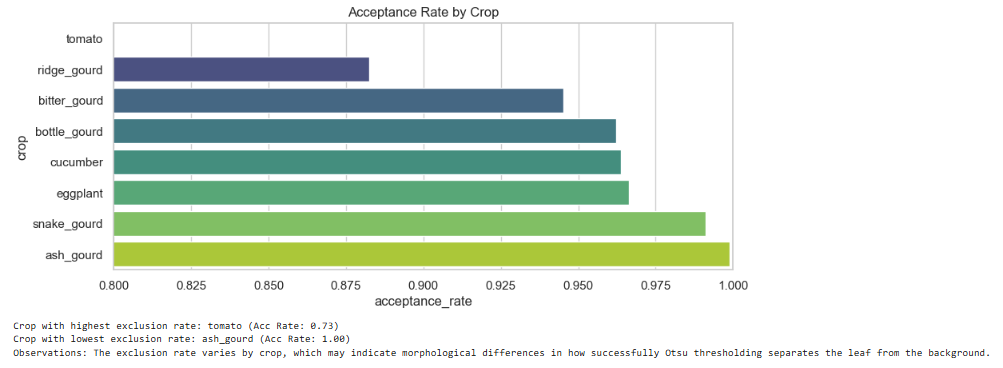
\includegraphics[width=0.95\linewidth]{haha.png}\\[5pt]
        {\scriptsize
        Acceptance varies across crops, with tomato showing the
        highest exclusion and ash\_gourd the highest acceptance.
        }

        % Right: Sanity checks
        \column{0.45\textwidth}
        \centering
        \textbf{Feature Sanity Checks}\\[10pt]

        \iconCheck\quad \textbf{NaN / Infinite Values}\\
        {\scriptsize 0 missing, 0 infinite}\\[10pt]

        \iconCheck\quad \textbf{Constant Features}\\
        {\scriptsize None found}\\[10pt]

        \iconCheck\quad \textbf{Duplicate Records}\\
        {\scriptsize Checked across accepted data}\\[10pt]

        \iconCheck\quad \textbf{Outliers}\\
        {\scriptsize Checked across feature distributions}

    \end{columns}

\end{frame}
% ============================================================
% FRAME: Feature Distributions
% ============================================================
\begin{frame}{Feature Distributions}
    \framesubtitle{Visual inspection of the 38 extracted features}

    \begin{center}
    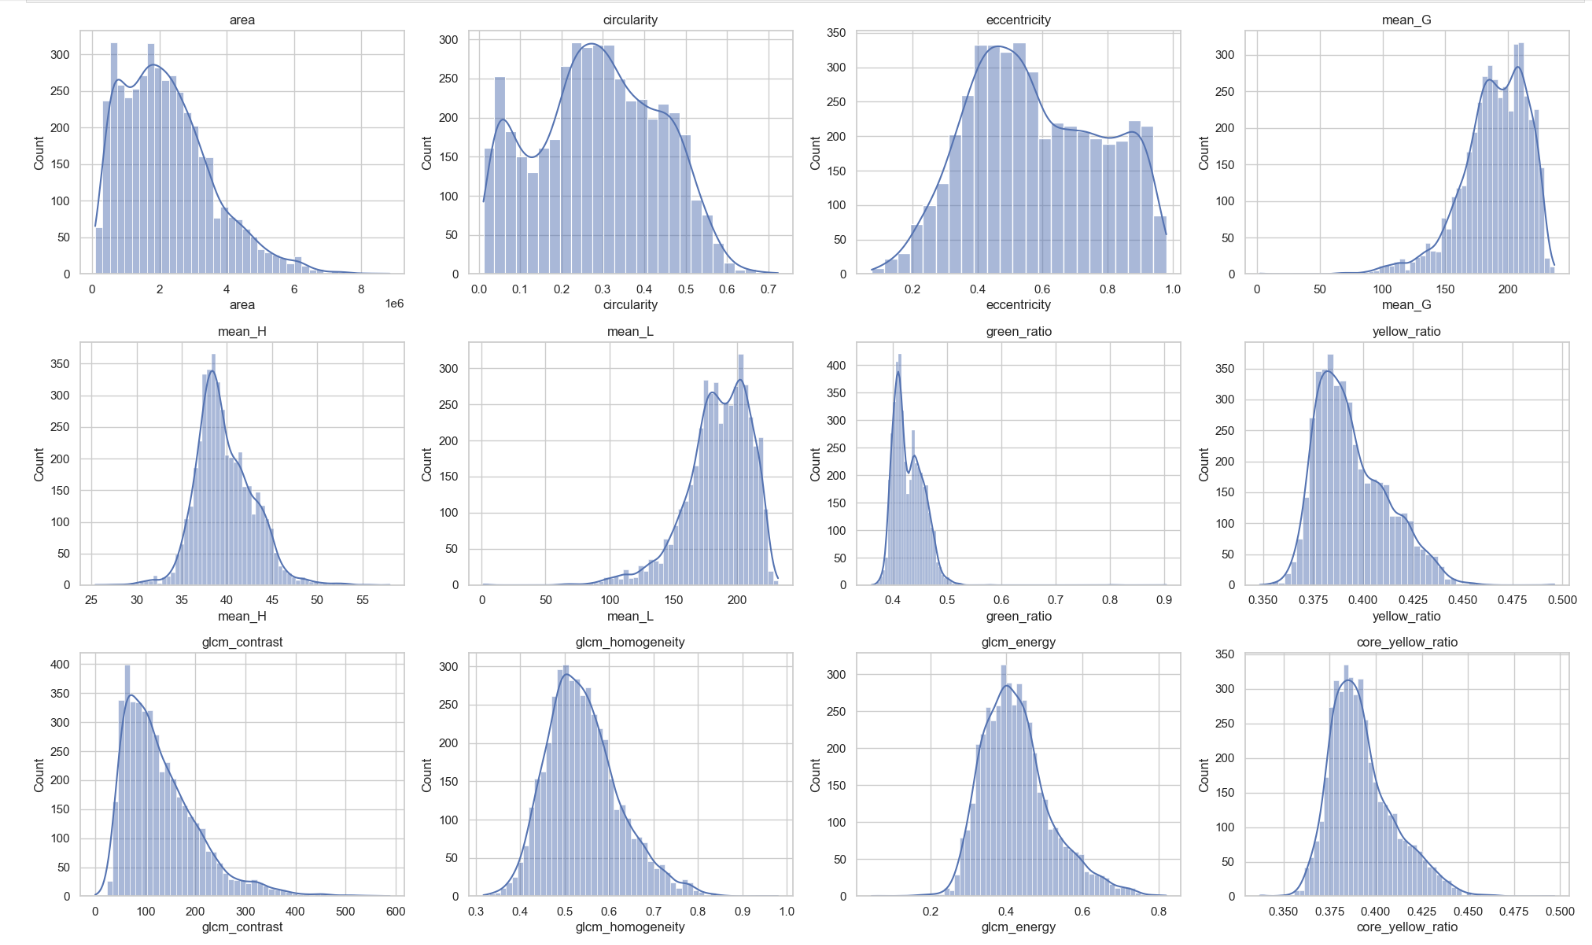
\includegraphics[width=0.92\textwidth]{feature_distributions.png}
    \end{center}

    \vspace{0.1cm}
    {\scriptsize\itshape Histograms of shape, color, and texture features
    across the accepted dataset -- used to confirm reasonable spread and
    absence of degenerate (constant or collapsed) distributions.}
\end{frame}
% ============================================================
% FRAME: Mask Area Distribution of Entire Dataset
% ============================================================
\begin{frame}{Mask Area Distribution of Entire Dataset}
    \framesubtitle{Population-level overview of segmentation area ratios}

    \begin{center}
        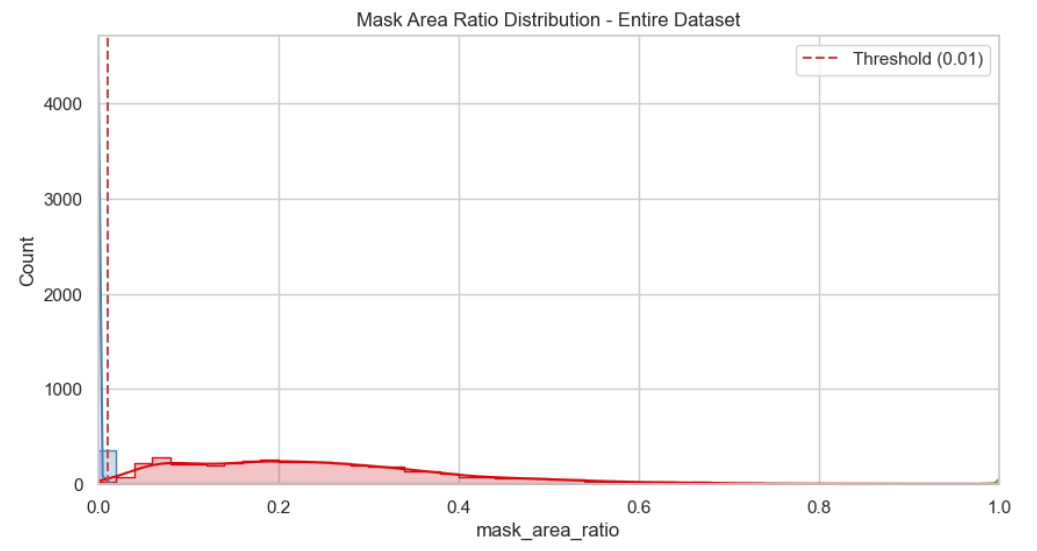
\includegraphics[width=0.78\textwidth, height=0.62\textheight, keepaspectratio]{wowow.png}
    \end{center}

    \vspace{-0.1cm}
    {\scriptsize\itshape Distribution across all samples illustrating leaf-to-image coverage ratios prior to downstream feature extraction and graph mapping.}
\end{frame}

% ============================================================
% FRAME: Dataset Filtering Summary
% ============================================================
\begin{frame}{Dataset Filtering Summary}
    \framesubtitle{Overall throughput after Otsu-based mask area validation}

    \begin{columns}[c]
        \column{0.52\textwidth}
        \begin{table}[]
            \centering
            \small
            \begin{tabular}{lr}
                \toprule
                \textbf{Metric} & \textbf{Value} \\
                \midrule
                Original Samples & 4,749 \\
                Accepted Samples & \textbf{\textcolor{green!60!black}{4,387}} \\
                Excluded Samples & \textbf{\textcolor{red}{362}} \\
                \midrule
                \textbf{Overall Acceptance Rate} & \textbf{92.38\%} \\
                \bottomrule
            \end{tabular}
        \end{table}

        \column{0.44\textwidth}
        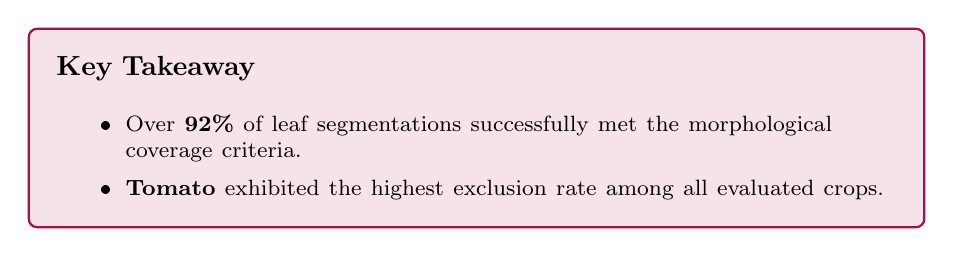
\begin{tikzpicture}
            \node[rectangle, draw=amritaMaroon, thick, fill=maroonSoft, 
                  rounded corners=3pt, inner sep=10pt, text width=0.88\textwidth] {
                \textbf{Key Takeaway}
                \vspace{0.2cm}\\
                \footnotesize
                \begin{itemize}\footnotesize
                    \item Over \textbf{92\%} of leaf segmentations successfully met the morphological coverage criteria.
                    \item \textbf{Tomato} exhibited the highest exclusion rate among all evaluated crops.
                \end{itemize}
            };
        \end{tikzpicture}
    \end{columns}

    \vspace{0.4cm}
    \begin{center}
        {\scriptsize\itshape High retention confirms the viability of automated thresholding while pruning failure modes before graph construction.}
    \end{center}
\end{frame}

% ============================================================
% FRAME: Continuous Feature Discretization
% ============================================================
\begin{frame}{Feature Discretization for Graph Labeling}
    \framesubtitle{Converting continuous morphological traits into discrete node labels}

    \textbf{Quantile-Based Discretization}
    \vspace{0.15cm}

    {\footnotesize To enable symbolic neighborhood aggregation in the \textbf{WL Graph Kernel}, continuous feature values are partitioned using \texttt{KBinsDiscretizer} (\texttt{strategy='quantile'}, $k=3$) \cite{pedregosa2011scikit, dougherty1995supervised}:}

    \vspace{0.3cm}
    \begin{itemize}\footnotesize
        \item \textbf{\texttt{low} ($[0, \frac{1}{3})$):} First quantile / lowest feature responses.
        \item \textbf{\texttt{medium} ($[\frac{1}{3}, \frac{2}{3}]$):} Interquartile / balanced feature responses.
        \item \textbf{\texttt{high} ($(\frac{2}{3}, 1]$):} Top quantile / dominant feature values.
    \end{itemize}

    \vspace{0.45cm}
    % \begin{tikzpicture}
    %     \node[rectangle, draw=amritaMaroon, very thick, fill=maroonSoft,
    %           rounded corners=3pt, inner sep=8pt, text width=0.92\textwidth] {
    %         \footnotesize
    %         \textbf{Impact on WL Initialization:} Continuous measurements (e.g., leaf area $\rightarrow 42.5\,\text{cm}^2$) are converted into discrete, categorical tokens (e.g., \texttt{LA\_low}, \texttt{LC\_high}) to initialize node labels prior to iterative neighborhood relabeling.
    %     };
    % \end{tikzpicture}
\end{frame}

% ============================================================
% FRAME: Evaluated Graph Representations
% ============================================================
\begin{frame}{Evaluated Graph Representations}


    \begin{columns}[T]
        \column{0.48\textwidth}
        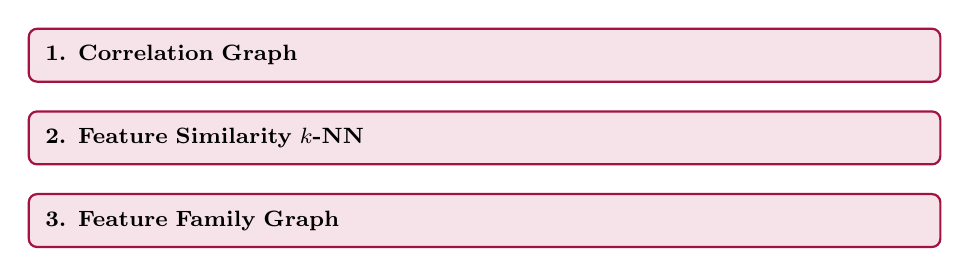
\begin{tikzpicture}[every node/.style={transform shape}]
            \tikzset{gbox/.style={draw=amritaMaroon, thick, fill=maroonSoft, rounded corners=3pt, text width=0.92\columnwidth, inner sep=6pt, font=\footnotesize}}

            \node[gbox] (g1) {\textbf{1. Correlation Graph}};
            \node[gbox, below=0.35cm of g1] (g2) {\textbf{2. Feature Similarity $k$-NN}};
            \node[gbox, below=0.35cm of g2] (g3) {\textbf{3. Feature Family Graph}};
        \end{tikzpicture}

        \column{0.48\textwidth}
        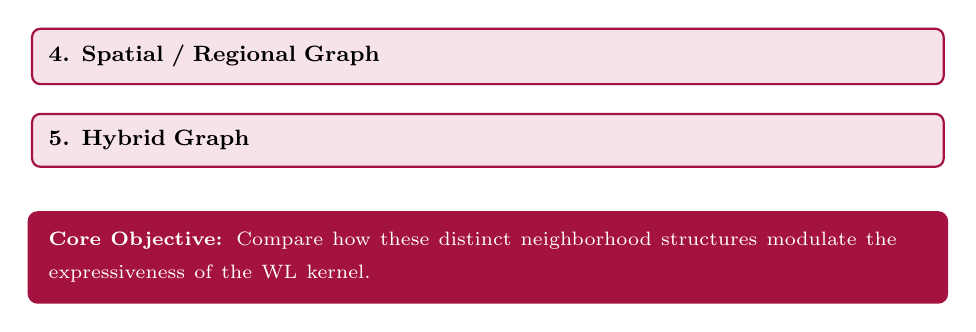
\begin{tikzpicture}[every node/.style={transform shape}]
            \tikzset{gbox/.style={draw=amritaMaroon, thick, fill=maroonSoft, rounded corners=3pt, text width=0.92\columnwidth, inner sep=6pt, font=\footnotesize}}

            \node[gbox] (g4) {\textbf{4. Spatial / Regional Graph}};
            \node[gbox, below=0.35cm of g4] (g5) {\textbf{5. Hybrid Graph}};

            \node[rectangle, draw=amritaMaroon, very thick, fill=amritaMaroon, text=white,
                  rounded corners=3pt, inner sep=7pt, text width=0.92\columnwidth, below=0.55cm of g5] {
                \scriptsize\textbf{Core Objective:} Compare how these distinct neighborhood structures modulate the expressiveness of the WL kernel.
            };
        \end{tikzpicture}
    \end{columns}
\end{frame}

% ============================================================
% FRAME: Correlation Graph Representation & Topology
% ============================================================
\begin{frame}{Correlation Graph Representation}
    \framesubtitle{Formulation, edge thresholding, and resulting topology}

    \begin{columns}[c]
        \column{0.50\textwidth}
        \textbf{Pearson Correlation Coefficient ($r$) \cite{pearson1895notes}}
        \vspace{0.05cm}

        {\scriptsize
        $$ r = \frac{\sum (X_i - \bar{X})(Y_i - \bar{Y})}{\sqrt{\sum (X_i - \bar{X})^2 \sum (Y_i - \bar{Y})^2}}, \quad r \in [-1, +1] $$
        }

        \vspace{0.1cm}
        \textbf{Edge Formation Criteria}
        \vspace{0.05cm}
        \begin{itemize}\scriptsize
            \item Connect features $u, v$ if \textbf{$|r| \ge \text{threshold}$}.
            \item Tested thresholds: \textbf{0.60, 0.70, 0.80, 0.90}.
        \end{itemize}

        \vspace{0.1cm}
        \textbf{Correlation Scale}
        \vspace{0.05cm}
        \begin{table}[]
            \centering
            \tiny
            \begin{tabular}{r p{3.6cm}}
                \toprule
                \textbf{$r$} & \textbf{Interpretation} \\
                \midrule
                $\pm 1.0$ & Perfect linear relationship \\
                $\pm 0.8$ & Strong positive / negative relation \\
                $0.0$ & No linear association \\
                \bottomrule
            \end{tabular}
        \end{table}

        \vspace{0.05cm}
        {\tiny\textbf{Example ($\tau = 0.80$):} $r=0.997 \rightarrow \text{Edge}$, $r=0.650 \rightarrow \text{No edge}$.}

        \column{0.50\textwidth}
        \centering
        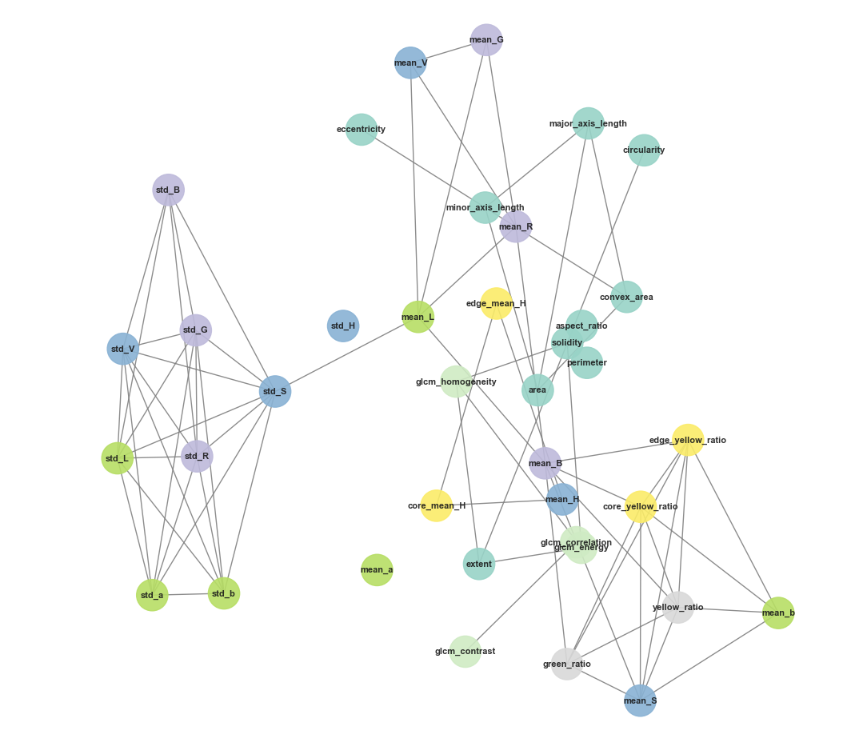
\includegraphics[width=\linewidth, height=0.75\textheight, keepaspectratio]{correlation_graph.png}
    \end{columns}
\end{frame}
% ============================================================
% FRAME: Feature-Similarity K-NN Graph Representation
% ============================================================
\begin{frame}{Feature-Similarity $K$-NN Graph}
    \framesubtitle{Data-driven neighborhood topology based on sample distributions \cite{cover1967nearest}}

    \begin{columns}[c]
        \column{0.50\textwidth}
        \textbf{Purpose}
        \vspace{0.05cm}

        {\scriptsize Link the \textbf{38 feature nodes} via non-linear distance metric proximity across training distributions.}

        \vspace{0.15cm}
        \textbf{Step-by-Step Construction}
        \vspace{0.05cm}
        \begin{itemize}\scriptsize
            \item \textbf{Vectorization:} Treat each trait as an $N$-dim vector across training instances.
            \item \textbf{Pairwise Metric:} Calculate metric distance between all feature pairs.
            \item \textbf{Top-$K$ Selection:} Identify each feature's $K$ closest neighbors.
            \item \textbf{Edge Insertion:} Connect nodes to their identified $K$ nearest neighbors.
        \end{itemize}

        \vspace{0.15cm}
        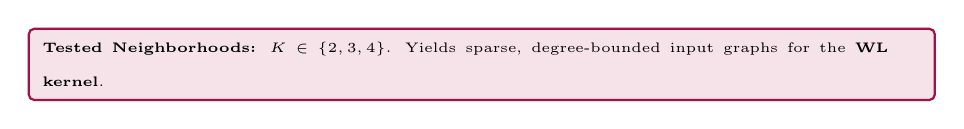
\begin{tikzpicture}
            \node[rectangle, draw=amritaMaroon, thick, fill=maroonSoft,
                  rounded corners=2pt, inner sep=5pt, text width=0.92\columnwidth] {
                \tiny\textbf{Tested Neighborhoods:} $K \in \{2, 3, 4\}$. Yields sparse, degree-bounded input graphs for the \textbf{WL kernel}.
            };
        \end{tikzpicture}

        \column{0.50\textwidth}
        \centering
        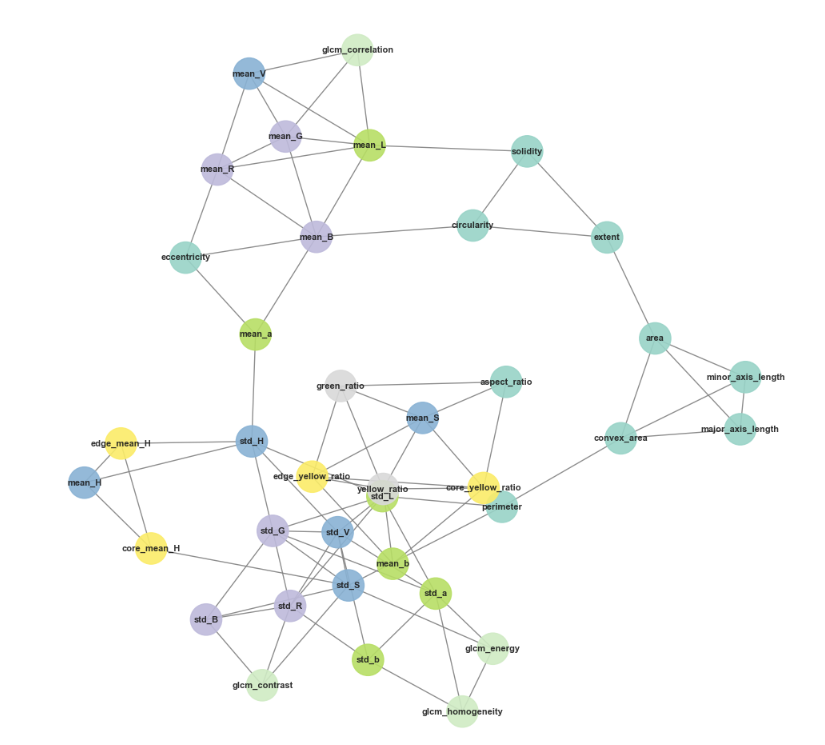
\includegraphics[width=\linewidth, height=0.75\textheight, keepaspectratio]{knn_Graph.png}
    \end{columns}
\end{frame}
% ============================================================
% FRAME: Feature Family Graph Representation
% ============================================================
\begin{frame}{Feature Family Graph}
    \framesubtitle{Category-based topology with cross-domain links}

    \begin{columns}[c]
        \column{0.56\textwidth}
        {\scriptsize\textbf{Purpose:} Group the 38 traits into domain cliques with cross-family links.}
        \vspace{0.15cm}

        \begin{table}[]
            \centering
            \fontsize{4.5pt}{5.5pt}\selectfont
            \begin{tabular}{p{1.7cm} p{3.7cm} r}
                \toprule
                \textbf{Category} & \textbf{Features} & \textbf{Count} \\
                \midrule
                Shape \& Geometry & area, perimeter, aspect\_ratio, circularity, extent, solidity, convex\_area, major\_axis\_length, minor\_axis\_length, eccentricity & 10 \\
                \midrule
                Global Color & mean/std of R, G, B, H, S, V, L, a, b; green\_ratio, yellow\_ratio & 20 \\
                \midrule
                Texture & glcm\_contrast, glcm\_homogeneity, glcm\_energy, glcm\_correlation \cite{haralick1973textural} & 4 \\
                \midrule
                Spatial / Regional & core\_mean\_H, core\_yellow\_ratio, edge\_mean\_H, edge\_yellow\_ratio & 4 \\
                \midrule
                \textbf{Total} & \textbf{All extracted leaf traits} & \textbf{38} \\
                \bottomrule
            \end{tabular}
        \end{table}

        \vspace{0.1cm}
        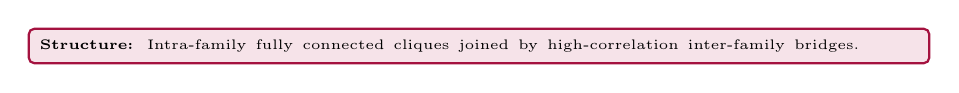
\begin{tikzpicture}
            \node[rectangle, draw=amritaMaroon, thick, fill=maroonSoft,
                  rounded corners=2pt, inner sep=4pt, text width=0.92\columnwidth] {
                \tiny\textbf{Structure:} Intra-family fully connected cliques joined by high-correlation inter-family bridges.
            };
        \end{tikzpicture}

        \column{0.44\textwidth}
        \centering
        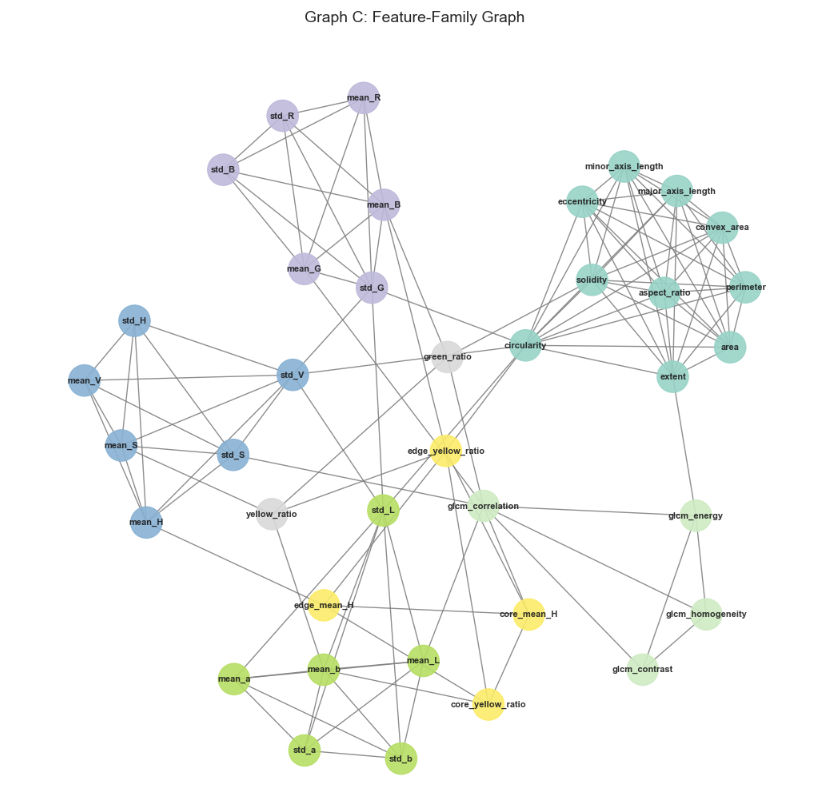
\includegraphics[width=\linewidth, height=0.75\textheight, keepaspectratio]{feature_family.png}
    \end{columns}
\end{frame}
% ============================================================
% FRAME: Spatial / Regional Graph
% ============================================================
\begin{frame}{Spatial / Regional Graph}
    \framesubtitle{Connecting core--edge features with correlated global features}

    \begin{columns}[T]

        % Left: Construction
        \column{0.47\textwidth}
        \textbf{Graph Construction}\\[4pt]

        {\footnotesize
        \textbf{38 feature nodes}, including 4 spatial features:
        }

        \begin{itemize}\footnotesize
            \item \texttt{core\_mean\_H}
            \item \texttt{core\_yellow\_ratio}
            \item \texttt{edge\_mean\_H}
            \item \texttt{edge\_yellow\_ratio}
        \end{itemize}

        \vspace{0.1cm}

        \begin{enumerate}\footnotesize
            \item \textbf{Core--Core:} Connect core features.
            \item \textbf{Edge--Edge:} Connect edge features.
            \item \textbf{Core--Edge:} Connect corresponding core and edge features.
            \item \textbf{Global--Spatial:} Connect the remaining 34 features when
            \[
            |\text{Pearson }r| \geq 0.60
            \]
        \end{enumerate}

        % \vspace{0.15cm}

        % \begin{tikzpicture}
        %     \node[rectangle, draw=amritaMaroon, thick, fill=maroonSoft,
        %           rounded corners=2pt, inner sep=5pt,
        %           text width=0.92\columnwidth] {
        %         \scriptsize
        %         \textbf{Key idea:} Fixed spatial relationships +
        %         correlation-based global connections.
        %     };
        % \end{tikzpicture}


        % Right: Visualization
        \column{0.53\textwidth}
        \centering
        \textbf{Resulting Spatial Graph}\\[5pt]

        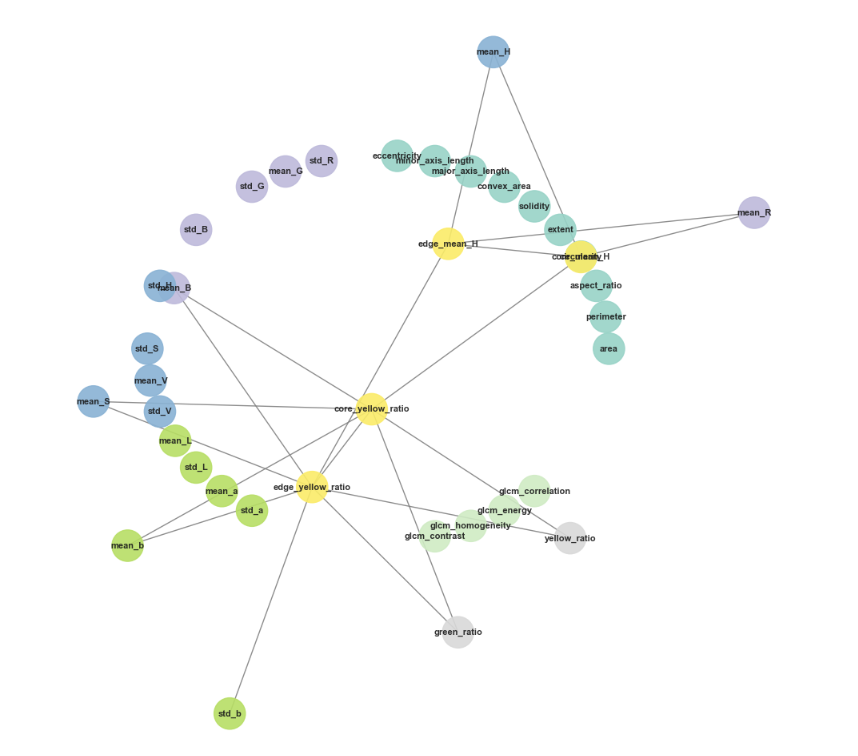
\includegraphics[
            width=\linewidth,
            height=0.70\textheight,
            keepaspectratio
        ]{spatial_graph.png}

    \end{columns}
\end{frame}
% ============================================================
% FRAME: Hybrid Graph
% ============================================================
\begin{frame}{Hybrid Graph}
    \framesubtitle{Combining correlation, feature-family, and spatial relationships}

    \begin{columns}[T]

        % Left: Construction
        \column{0.47\textwidth}
        \textbf{Graph Construction}\\[5pt]

        {\footnotesize
        \textbf{38 feature nodes} formed by combining three graph structures:
        }

        \begin{itemize}\footnotesize
            \item \textbf{Correlation:}
            \[
            |\text{Pearson }r| \geq 0.80
            \]

            \item \textbf{Feature Family:}\\
            Connects features within their predefined families.

            \item \textbf{Spatial:}\\
            Preserves core--edge relationships with
            \[
            |\text{Pearson }r| \geq 0.70
            \]
        \end{itemize}

        \vspace{0.05cm}

        % \begin{tikzpicture}
        %     \node[rectangle, draw=amritaMaroon, thick, fill=maroonSoft,
        %           rounded corners=2pt, inner sep=5pt,
        %           text width=0.92\columnwidth] {
        %         \scriptsize
        %         \textbf{Fusion:} All edges are merged into one
        %         unified graph. Edges supported by multiple
        %         components are marked as \textbf{multiple}.
        %     };
        % \end{tikzpicture}


        % Right: Visualization
        \column{0.53\textwidth}
        \centering
        \textbf{Resulting Hybrid Graph}\\[5pt]

        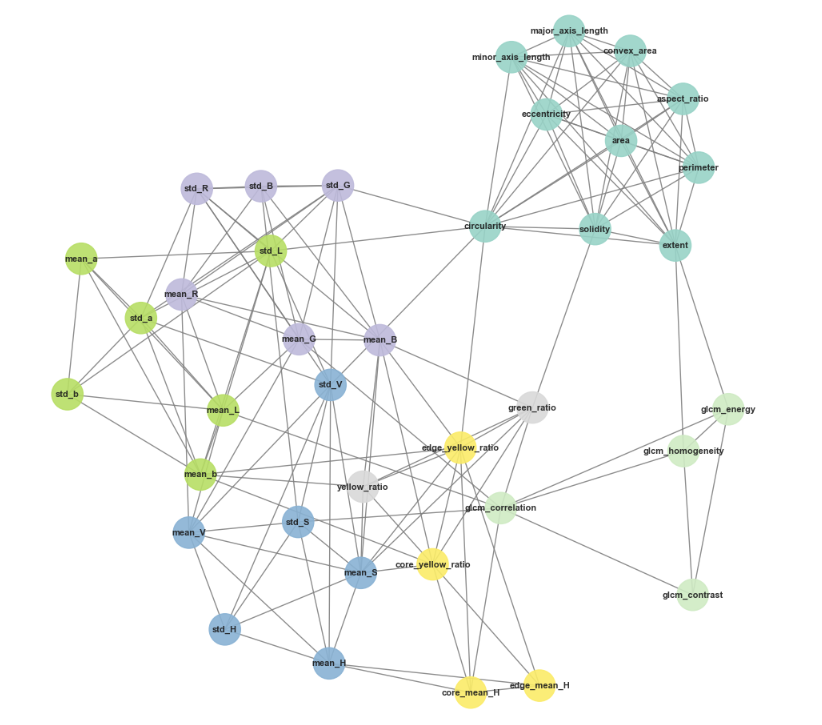
\includegraphics[
            width=\linewidth,
            height=0.70\textheight,
            keepaspectratio
        ]{hybrid_graph.png}

    \end{columns}
\end{frame}
% ============================================================
% FRAME: WL Iterations & Subtree Feature Vector (1/2)
% ============================================================
\begin{frame}{WL Iterations: Neighborhood Propagation}
    \framesubtitle{Iterative label refinement from local features to larger subtrees \cite{shervashidze2011weisfeiler}}

    \begin{columns}[T]
        \column{0.48\textwidth}
        \textbf{1. Initial Node Labelling ($h = 0$)}
        \vspace{0.15cm}
        \begin{itemize}\footnotesize
            \item Each leaf is structured as a graph with \textbf{38 feature nodes}.
            \item Continuous feature values are mapped to categorical bins: \textbf{Low}, \textbf{Medium}, or \textbf{High}.
            \item These form the baseline node labels ($h = 0$).
        \end{itemize}

        \vspace{0.3cm}
        \textbf{2. First Iteration ($h = 1$)}
        \vspace{0.15cm}
        \begin{itemize}\footnotesize
            \item For each node, WL aggregates:
            \begin{center}
                \scriptsize\texttt{Current Label} $+$ \texttt{Multiset of Neighbor Labels}
            \end{center}
            \item The combined string forms a \textbf{neighborhood signature}.
            \item Signatures are compressed into new, unique WL labels, capturing 1-hop local topology.
        \end{itemize}

        \column{0.48\textwidth}
        \textbf{3. Higher-Order Iterations ($h = 2, 3$)}
        \vspace{0.15cm}
        \begin{itemize}\footnotesize
            \item Output labels from iteration $h-1$ serve directly as input for iteration $h$.
            \item The multiset aggregation is repeated sequentially for depths \textbf{$h = 2$} and \textbf{$h = 3$}.
            \item With each hop, the compressed label captures an expanding subtree receptive field around each feature node.
        \end{itemize}

        \vspace{0.35cm}
        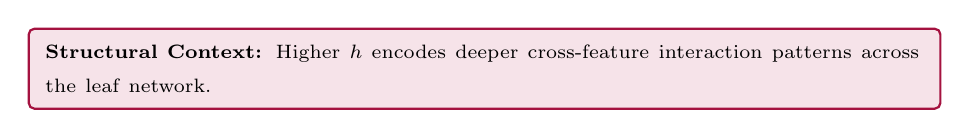
\begin{tikzpicture}
            \node[rectangle, draw=amritaMaroon, thick, fill=maroonSoft,
                  rounded corners=2pt, inner sep=6pt, text width=0.92\columnwidth] {
                \scriptsize\textbf{Structural Context:} Higher $h$ encodes deeper cross-feature interaction patterns across the leaf network.
            };
        \end{tikzpicture}
    \end{columns}
\end{frame}

% ============================================================
% FRAME: WL Iterations & Subtree Feature Vector (2/2)
% ============================================================
\begin{frame}{Generating the WL Subtree Feature Vector}
    \framesubtitle{Constructing the final numerical embedding for classification \cite{shervashidze2011weisfeiler}}

    \begin{columns}[c]
        \column{0.52\textwidth}
        \textbf{Vector Construction Workflow}
        \vspace{0.15cm}
        \begin{itemize}\footnotesize
            \item \textbf{Label Histogramming:} At each height ($h = 0, 1, 2, 3$), all generated unique labels across the graph are counted.
            \item \textbf{Feature Concatenation:} The label frequencies from all iterations are accumulated into a single global vector:
            \begin{center}
                \scriptsize $\phi(G) = \big[\mathbf{c}_0(G) \,\|\, \mathbf{c}_1(G) \,\|\, \mathbf{c}_2(G) \,\|\, \mathbf{c}_3(G)\big]$
            \end{center}
            \item \textbf{Embedding Interpretation:} The vector measures the precise occurrence frequencies of distinct subtree patterns within the leaf graph.
        \end{itemize}

        \column{0.44\textwidth}
        \centering
        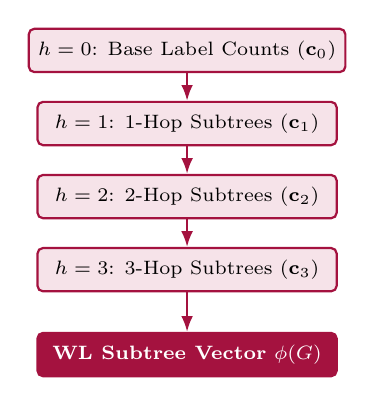
\begin{tikzpicture}[every node/.style={transform shape}]
            \tikzset{vecstep/.style={rectangle, draw=amritaMaroon, thick, fill=maroonSoft,
                     rounded corners=2pt, minimum width=3.8cm, minimum height=0.55cm, font=\scriptsize, align=center}}
            
            \node[vecstep] (s0) {$h=0$: Base Label Counts ($\mathbf{c}_0$)};
            \node[vecstep, below=0.35cm of s0] (s1) {$h=1$: 1-Hop Subtrees ($\mathbf{c}_1$)};
            \node[vecstep, below=0.35cm of s1] (s2) {$h=2$: 2-Hop Subtrees ($\mathbf{c}_2$)};
            \node[vecstep, below=0.35cm of s2] (s3) {$h=3$: 3-Hop Subtrees ($\mathbf{c}_3$)};
            \node[vecstep, fill=amritaMaroon, text=white, below=0.5cm of s3] (vec) {\textbf{WL Subtree Vector} $\phi(G)$};

            \draw[-{Latex[length=2mm]}, thick, draw=amritaMaroon] (s0) -- (s1);
            \draw[-{Latex[length=2mm]}, thick, draw=amritaMaroon] (s1) -- (s2);
            \draw[-{Latex[length=2mm]}, thick, draw=amritaMaroon] (s2) -- (s3);
            \draw[-{Latex[length=2mm]}, thick, draw=amritaMaroon] (s3) -- (vec);
        \end{tikzpicture}
    \end{columns}

    \vspace{0.35cm}
    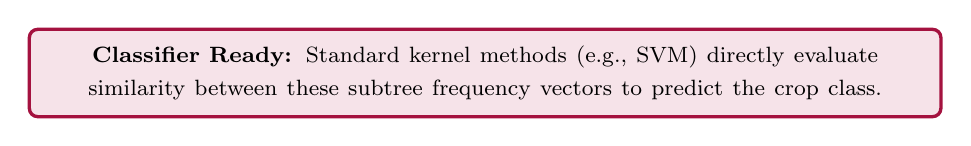
\begin{tikzpicture}
        \node[rectangle, draw=amritaMaroon, very thick, fill=maroonSoft,
              rounded corners=3pt, inner sep=6pt, text width=0.92\textwidth, align=center] {
            \footnotesize\textbf{Classifier Ready:} Standard kernel methods (e.g., SVM) directly evaluate similarity between these subtree frequency vectors to predict the crop class.
        };
    \end{tikzpicture}
\end{frame}

% ============================================================
% FRAME: WL Subtree Feature Representations & Kernel Construction
% ============================================================
\begin{frame}{WL Subtree Representations \& Kernel Matrix}
    \framesubtitle{From label frequency vectors to pairwise graph similarity matrices \cite{shervashidze2011weisfeiler, scholkopf2002learning}}

    \begin{columns}[T]
        \column{0.48\textwidth}
        \textbf{1. Subtree Feature Matrix ($\Phi$)}
        \vspace{0.15cm}

        \begin{itemize}\footnotesize
            \item Each leaf image is represented by a discrete \textbf{WL subtree feature vector}.
            \item Elements correspond to occurrence frequencies of unique WL labels accumulated across iterations ($h = 0, 1, 2, 3$).
            \item Stacking all sample vectors yields the global representation matrix $\Phi$.
        \end{itemize}

        \vspace{0.3cm}
        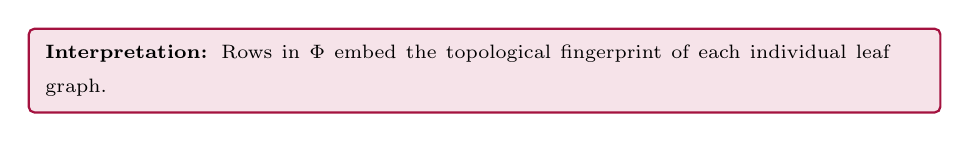
\begin{tikzpicture}
            \node[rectangle, draw=amritaMaroon, thick, fill=maroonSoft,
                  rounded corners=2pt, inner sep=6pt, text width=0.92\columnwidth] {
                \scriptsize\textbf{Interpretation:} Rows in $\Phi$ embed the topological fingerprint of each individual leaf graph.
            };
        \end{tikzpicture}

        \column{0.48\textwidth}
        \textbf{2. Kernel Matrix Construction}
        \vspace{0.15cm}

        {\footnotesize Computed via inner products of the WL feature matrices:}

        \vspace{0.2cm}
        \textbf{Training Kernel Matrix:}
        \begin{equation*}
            K_{\text{train}} = \Phi_{\text{train}} \Phi_{\text{train}}^T
        \end{equation*}
        {\scriptsize Evaluates pairwise similarity across all training leaf graphs.}

        \vspace{0.25cm}
        \textbf{Validation Kernel Matrix:}
        \begin{equation*}
            K_{\text{val}} = \Phi_{\text{val}} \Phi_{\text{train}}^T
        \end{equation*}
        {\scriptsize Measures similarity between unseen validation graphs and the training basis.}
    \end{columns}

    \vspace{0.35cm}
    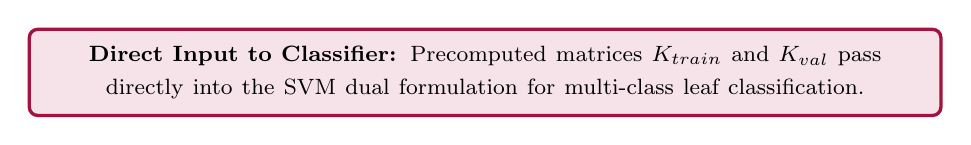
\begin{tikzpicture}
        \node[rectangle, draw=amritaMaroon, very thick, fill=maroonSoft,
              rounded corners=3pt, inner sep=6pt, text width=0.92\textwidth, align=center] {
            \footnotesize\textbf{Direct Input to Classifier:} Precomputed matrices $K_{\text{train}}$ and $K_{\text{val}}$ pass directly into the SVM dual formulation for multi-class leaf classification.
        };
    \end{tikzpicture}
\end{frame}
% ============================================================
% FRAME: Kernel Normalization
% ============================================================
\begin{frame}{Kernel Normalization}
    \framesubtitle{Standardizing similarity scales across sample feature lengths \cite{scholkopf2002learning}}

    \begin{columns}[T]
        \column{0.52\textwidth}
        \textbf{Cosine-Style Normalization Formula \cite{scholkopf2002learning}}
        \vspace{0.1cm}
        \begin{equation*}
            K_{\text{norm}}(i,j) = \frac{K(i,j)}{\sqrt{K(i,i) \cdot K(j,j)}}
        \end{equation*}

        \vspace{0.1cm}
        \begin{itemize}\scriptsize
            \item $K(i,j)$: Pairwise similarity between samples $i$ and $j$.
            \item $K(i,i)$, $K(j,j)$: Self-similarity (inner-product norms).
            \item Converts raw counts into bounded metric space; eliminates bias from feature vector scale differences.
        \end{itemize}

        \column{0.44\textwidth}
        \textbf{Train vs. Validation Behavior}
        \vspace{0.15cm}

        \begin{itemize}\footnotesize
            \item \textbf{Training Matrix ($K_{\text{train}}$):} \\
            Square ($N_{\text{train}} \times N_{\text{train}}$). Diagonal entries scale to:
            \begin{center}
                \small\bfseries $K_{\text{norm}}(i,i) \approx 1.0$
            \end{center}
            \item \textbf{Validation Matrix ($K_{\text{val}}$):} \\
            Rectangular ($N_{\text{val}} \times N_{\text{train}}$). Evaluates unseen graphs against training anchors; diagonal is not $1$.
        \end{itemize}
    \end{columns}

    \vspace{0.3cm}
    \begin{center}
        
\begin{tikzpicture}[node distance=0.4cm, auto, >=Latex]
            \tikzset{flowstep/.style={draw=amritaMaroon, thick, fill=maroonSoft, rounded corners=2pt, font=\tiny, inner sep=3pt, align=center}}
            \node[flowstep] (f1) {WL Subtree\\Vectors};
            \node[flowstep, right=0.35cm of f1] (f2) {Raw Kernels\\{\tiny $K_{\text{tr}}, K_{\text{val}}$}};
            \node[flowstep, right=0.35cm of f2] (f3) {Diagonal-Based\\Normalization};
            \node[flowstep, fill=amritaMaroon, text=white, right=0.35cm of f3] (f4) {Normalized\\Kernel Matrices};

            \draw[->, thick, draw=amritaMaroon] (f1) -- (f2);
            \draw[->, thick, draw=amritaMaroon] (f2) -- (f3);
            \draw[->, thick, draw=amritaMaroon] (f3) -- (f4);
        \end{tikzpicture}
    \end{center}
\end{frame}

% % ============================================================
% % FRAME: Why Use the WL Kernel?
% % ============================================================
% \begin{frame}{Why Use the WL Kernel?}
%     \framesubtitle{Bridging structured leaf topology with kernelized decision boundaries}

%     \textbf{The Core Problem It Solves}
%     \vspace{0.1cm}

%     {\footnotesize Standard classifiers take flat tabular vectors and ignore interactions. The WL kernel converts relational graphs into structural similarity metrics.}

%     \vspace{0.3cm}
%     \begin{center}
%         \begin{tikzpicture}[node distance=0.5cm, auto, >=Latex]
%             \tikzset{pipenode/.style={draw=amritaMaroon, thick, fill=maroonSoft, rounded corners=2pt, font=\scriptsize, inner sep=4pt, align=center}}
%             \node[pipenode] (p1) {Leaf Image};
%             \node[pipenode, right=0.35cm of p1] (p2) {38 Feature Nodes\\(Graph $G$)};
%             \node[pipenode, right=0.35cm of p1] (p2) {38 Feature\\Nodes ($G$)};
%             \node[pipenode, right=0.35cm of p2] (p3) {WL Label\\Refinement};
%             \node[pipenode, right=0.35cm of p3] (p4) {Subtree Vector\\$\Phi(G)$};
%             \node[pipenode, fill=amritaMaroon, text=white, right=0.35cm of p4] (p5) {Kernel Similarity\\$K(G_i, G_j)$};

%             \draw[->, thick, draw=amritaMaroon] (p1) -- (p2);
%             \draw[->, thick, draw=amritaMaroon] (p2) -- (p3);
%             \draw[->, thick, draw=amritaMaroon] (p3) -- (p4);
%             \draw[->, thick, draw=amritaMaroon] (p4) -- (p5);
%         \end{tikzpicture}
%     \end{center}

%     \vspace{0.35cm}
%     \begin{columns}[c]
%         \column{0.48\textwidth}
%         \begin{tikzpicture}
%             \node[rectangle, draw=amritaMaroon, thick, fill=maroonSoft,
%                   rounded corners=2pt, inner sep=6pt, text width=0.92\columnwidth] {
%                 \footnotesize\textbf{Structural Query:}
%                 \vspace{0.1cm}\\
%                 \scriptsize \textit{“How structurally identical are two leaves based on the distribution of their multi-hop trait subtrees?”}
%             };
%         \end{tikzpicture}

%         \column{0.48\textwidth}
%         \begin{itemize}\footnotesize
%             \item \textbf{Input Distinction:} The downstream classifier does \textbf{not} see the original 38 features.
%             \item \textbf{Topological Input:} It operates entirely on graph-to-graph similarity values provided by $K_{\text{norm}}$.
%         \end{itemize}
%     \end{columns}
% \end{frame}

% ============================================================
% FRAME: SVM Classification Workflow
% ============================================================
\begin{frame}{SVM Classification Pipeline}
    \framesubtitle{Evaluating precomputed kernel matrices within each cross-validation fold}

    \begin{columns}[T]
        \column{0.48\textwidth}
        \textbf{Step-by-Step Fold Execution}
        \vspace{0.15cm}

        \begin{enumerate}\scriptsize
            \item \textbf{Training Graphs:} Extract 38 features $\rightarrow$ construct graphs $\rightarrow$ run WL $\rightarrow$ compute $\Phi_{\text{train}}$ \cite{shervashidze2011weisfeiler}.
            \item \textbf{Train Kernel Matrix:}
            \begin{equation*}
                K_{\text{train}} = \Phi_{\text{train}}\Phi_{\text{train}}^T \quad (N_{\text{train}} \times N_{\text{train}})
            \end{equation*}
            \item \textbf{Validation Graphs:} Process validation leaves through identical discretization and WL vocabulary $\rightarrow$ $\Phi_{\text{val}}$.
            \item \textbf{Validation Kernel Matrix:}
            \begin{equation*}
                K_{\text{val}} = \Phi_{\text{val}}\Phi_{\text{train}}^T \quad (N_{\text{val}} \times N_{\text{train}})
            \end{equation*}
            \item \textbf{SVM Solver \cite{cortes1995support, chang2011libsvm}:} Fit dual SVM on $K_{\text{train}}$; evaluate target labels on $K_{\text{val}}$.
        \end{enumerate}

        \column{0.48\textwidth}
        \textbf{Target Classes}
        \vspace{0.15cm}

        {\footnotesize The SVM separates two primary physiological conditions:}
        \begin{center}
            \colorbox{maroonSoft}{\textbf{\texttt{NON-STRESSED}}} \quad vs. \quad \colorbox{amritaMaroon}{\textcolor{white}{\textbf{\texttt{STRESSED}}}}
        \end{center}

        \vspace{0.25cm}
        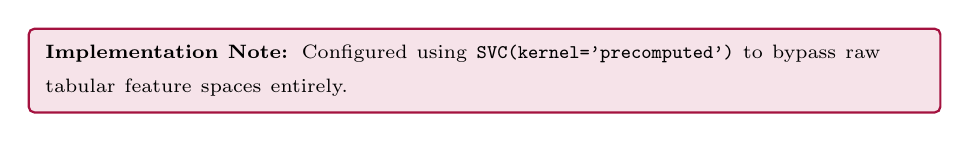
\begin{tikzpicture}
            \node[rectangle, draw=amritaMaroon, thick, fill=maroonSoft,
                  rounded corners=2pt, inner sep=6pt, text width=0.92\columnwidth] {
                \scriptsize\textbf{Implementation Note:} Configured using \texttt{SVC(kernel='precomputed')} to bypass raw tabular feature spaces entirely.
            };
        \end{tikzpicture}
    \end{columns}
\end{frame}

% % ============================================================
% % FRAME: Role Separation & Viva Explanation
% % ============================================================
% \begin{frame}{Role Separation: Methodology Architecture}
%     \framesubtitle{Clear functional division between pipeline components}

%     \begin{table}[]
%         \centering
%         \scriptsize
%         \begin{tabular}{p{3.2cm} p{6.8cm}}
%             \toprule
%             \textbf{Component} & \textbf{Core Function} \\
%             \midrule
%             38 Extracted Features & Quantify physical leaf morphology, color, texture, and regions. \\
%             Graph Construction & Defines structural topologies and inter-trait relationships. \\
%             WL Algorithm & Captures local and multi-hop subtree structures via relabeling. \\
%             WL Subtree Vector ($\Phi$) & High-dimensional numerical count of discovered graph subtrees. \\
%             WL Kernel ($K$) & Quantifies pairwise structural similarity between leaf graphs. \\
%             SVM Classifier & Learns the optimal maximum-margin hyperplane for stress labels. \\
%             \bottomrule
%         \end{tabular}
%     \end{table}

%     \vspace{0.25cm}
%     \begin{tikzpicture}
%         \node[rectangle, draw=amritaMaroon, very thick, fill=maroonSoft,
%               rounded corners=3pt, inner sep=7pt, text width=0.92\textwidth] {
%             \footnotesize
%             \textbf{Key Takeaway:} \textit{“WL extracts structural patterns from the feature graph, the kernel calculates similarity between those patterns, and the SVM uses these similarities to classify leaves as stressed or non-stressed.”}
%         };
%     \end{tikzpicture}
% \end{frame}

% % ============================================================
% % FRAME: Experimental Evaluation Setup
% % ============================================================
% \begin{frame}{Experimental Evaluation Configuration}
%     \framesubtitle{Comprehensive grid evaluation across topologies, depths, and folds}

%     \begin{columns}[c]
%         \column{0.50\textwidth}
%         \textbf{Evaluation Grid Dimensions}
%         \vspace{0.2cm}

%         \begin{itemize}\footnotesize
%             \item \textbf{5 Graph Topologies:}
%             \begin{itemize}\scriptsize
%                 \item Correlation Graph
%                 \item Feature-Similarity $k$-NN Graph
%                 \item Feature Family Graph
%                 \item Spatial / Regional Graph
%                 \item Hybrid Graph
%             \end{itemize}
%             \vspace{0.15cm}
%             \item \textbf{4 WL Subtree Heights:}
%             \begin{itemize}\scriptsize
%                 \item $h \in \{0, 1, 2, 3\}$
%             \end{itemize}
%             \vspace{0.15cm}
%             \item \textbf{Validation Protocol:}
%             \begin{itemize}\scriptsize
%                 \item Stratified 5-Fold Cross-Validation
%             \end{itemize}
%         \end{itemize}

%         \column{0.46\textwidth}
%         \centering
%         \begin{tikzpicture}[every node/.style={transform shape}]
%             \node[stepbox, fill=maroonSoft, minimum width=4.0cm] (m1) {\textbf{5 Graph Types}};
%             \node[stepbox, fill=maroonSoft, minimum width=4.0cm, below=0.25cm of m1] (m2) {\textbf{4 WL Heights ($h=0..3$)}};
%             \node[stepbox, fill=maroonSoft, minimum width=4.0cm, below=0.25cm of m2] (m3) {\textbf{5 Validation Folds}};
            
%             \node[stepbox, fill=amritaMaroon, text=white, minimum width=4.0cm, below=0.4cm of m3] (tot) {
%                 \textbf{Total Evaluations: 100} \\
%                 {\tiny $5 \times 4 \times 5 = 100\text{ Fold Experiments}$}
%             };

%             \draw[-{Latex[length=2mm]}, thick, draw=amritaMaroon] (m1) -- (m2);
%             \draw[-{Latex[length=2mm]}, thick, draw=amritaMaroon] (m2) -- (m3);
%             \draw[-{Latex[length=2mm]}, thick, draw=amritaMaroon] (m3) -- (tot);
%         \end{tikzpicture}
%     \end{columns}
% \end{frame}

% ============================================================
% FRAME: Model Evaluation (Testing on Folds)
% ============================================================
\begin{frame}{Model Evaluation \& Performance Metrics}
    \framesubtitle{Evaluating the SVM via K-Fold Cross-Validation \cite{kohavi1995study}}

    \textbf{1. K-Fold Cross-Validation \cite{kohavi1995study}}
    \vspace{0.1cm}

    \vspace{0.3cm}
    \begin{center}
    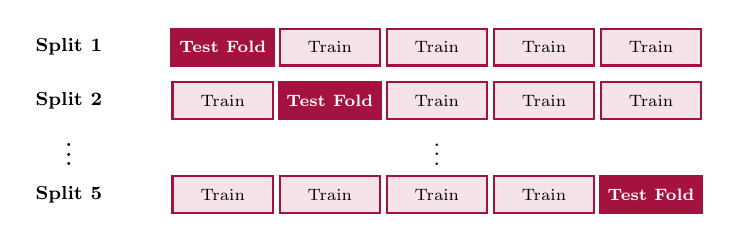
\begin{tikzpicture}[scale=0.85, every node/.style={transform shape}]
        \tikzset{
            fold/.style={rectangle, draw=amritaMaroon, thick, minimum width=1.5cm, minimum height=0.55cm, font=\scriptsize, align=center},
            train/.style={fold, fill=maroonSoft},
            test/.style={fold, fill=amritaMaroon, text=white, font=\scriptsize\bfseries}
        }
        
        % Split 1
        \node[font=\footnotesize\bfseries] at (-2.3, 0) {Split 1};
        \node[test]  at (0,0) {Test Fold};
        \node[train] at (1.6,0) {Train};
        \node[train] at (3.2,0) {Train};
        \node[train] at (4.8,0) {Train};
        \node[train] at (6.4,0) {Train};

        % Split 2
        \node[font=\footnotesize\bfseries] at (-2.3, -0.8) {Split 2};
        \node[train] at (0,-0.8) {Train};
        \node[test]  at (1.6,-0.8) {Test Fold};
        \node[train] at (3.2,-0.8) {Train};
        \node[train] at (4.8,-0.8) {Train};
        \node[train] at (6.4,-0.8) {Train};

        % Dots
        \node[font=\footnotesize\bfseries] at (-2.3, -1.5) {\vdots};
        \node at (3.2, -1.5) {\vdots};

        % Split K
        \node[font=\footnotesize\bfseries] at (-2.3, -2.2) {Split 5};
        \node[train] at (0,-2.2) {Train};
        \node[train] at (1.6,-2.2) {Train};
        \node[train] at (3.2,-2.2) {Train};
        \node[train] at (4.8,-2.2) {Train};
        \node[test]  at (6.4,-2.2) {Test Fold};
    \end{tikzpicture}
    \end{center}

    \vspace{0.3cm}
    \textbf{2. Calculating Metrics}
    \vspace{0.05cm}

    {\footnotesize For each test fold, we calculate standard performance metrics, which are then averaged to determine the final model performance:}
    \begin{itemize}\scriptsize
        \item \textbf{Accuracy:} Overall correctness of the model across all classes.
        \item \textbf{Precision:} Out of all plants predicted as a specific class, how many actually belonged to it.
        \item \textbf{Recall:} Out of all actual plants in a class, how many did the model find.
        \item \textbf{F1-Score:} The harmonic mean of Precision and Recall.
    \end{itemize}
\end{frame}

% ============================================================
% FRAME: Classification Results (Side-by-Side)
% ============================================================
\begin{frame}{Classification Results}
    \begin{columns}[c]
        \column{0.48\textwidth}
        \centering
        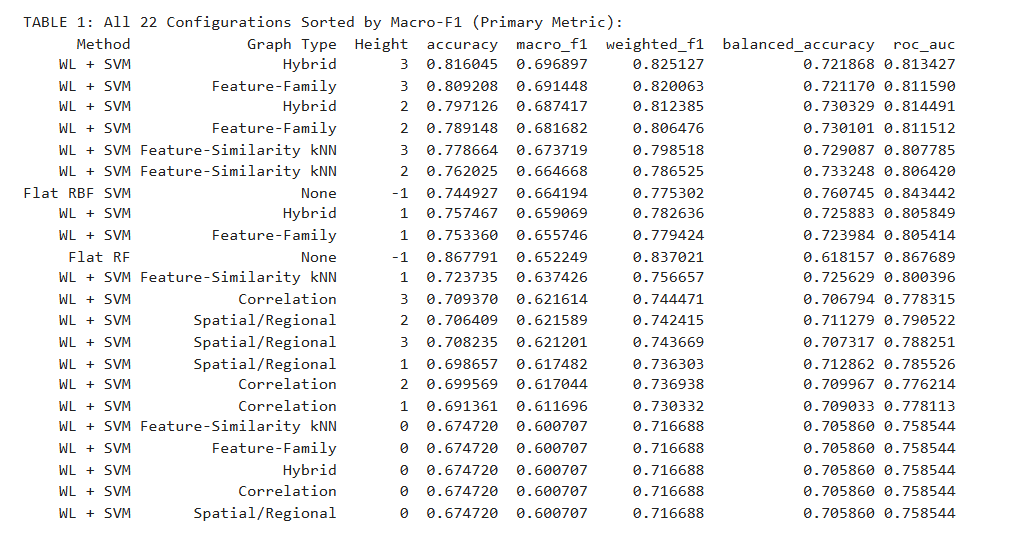
\includegraphics[width=\textwidth, height=0.75\textheight, keepaspectratio]{results1}
        
        \column{0.48\textwidth}
        \centering
        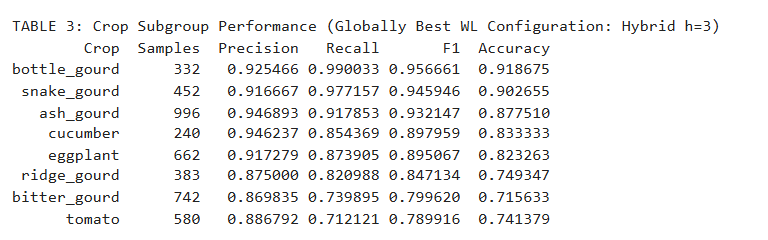
\includegraphics[width=\textwidth, height=0.75\textheight, keepaspectratio]{results2}
    \end{columns}
\end{frame}

% ============================================================
% FRAME: References
% ============================================================
\section{References}
\begin{frame}[allowframebreaks]{References}
    \tiny
    \bibliographystyle{IEEEtran}
    \bibliography{ref}
\end{frame}

% ============================================================
% FRAME: Thank You
% ============================================================
\begin{frame}
    \centering
    \vspace{1.5cm}
    {\Huge \textbf{\textcolor{amritaMaroon}{Thank You}}} \\[0.8cm]
    {\large \textbf{Questions \& Discussion}}
\end{frame}

\end{document}